% encoding: utf8
% !TEX encoding = utf8
% !TeX spellcheck = pl_PL

\chapter{Środowisko badawcze\label{chap:srodowisko}}
	\section{Budowa ogólna}
	Środowiskiem badawczym jest robot usługowy Velma (rys. \ref{fig:velma}) \cite{bib:velma2}, \cite{velma}. Został zaprojektowany i~wykonany przez Zespół Programowania Robotów i~Systemów Rozpoznających\cite{bib:robotyka}. Do obrotowego korpusu przytwierdzono dwa ramiona robotyczne Kuka LWR-4+\cite{bib:kukaPage} \cite{bib:kuka}. Mają siedem stopni swobody i~udźwig 7 kg. Na ich końcach znajdują się chwytaki Barretta\cite{bib:barrett}  oraz nadgarstkowe czujniki FTS (ang. Force Torque Sensor). Głowa robota umieszczona jest na dedykowanej konstrukcji która za pomocą dwóch silników elektrycznych pozwala na zginanie i~obrót głowy\cite{bib:velmaLeb} \cite{bib:velmaKorp}. Robot wyposażony jest w~czujnik wizyjny Microsoft Kinect oraz dwie kamery połączone w~stereoparę. Do głowy zamocowano mikrofon. Podzespoły robota są połączone z~komputerem sterującym przy pomocy magistral czasu rzeczywistego
	
	System sterowania o~twardych ograniczeniach czasowych pracuje z~częstotliwością 500 Hz. Struktura oprogramowania została stworzona w~oparciu o~teorię agentową. Oprogramowanie robota pisane jest przy wykorzystaniu struktury ramowej FABRIC. Programy nadzoruje system Linux z~nakładką Linux-RT. Dostępny jest symulator robota stworzony w~przy wykorzystaniu Gazebo i~silnika fizyki DART. 
	
	\begin{figure}
		\centering
		\subfigure[Zdjęcie robota]{
			\label{fig:velma1}
			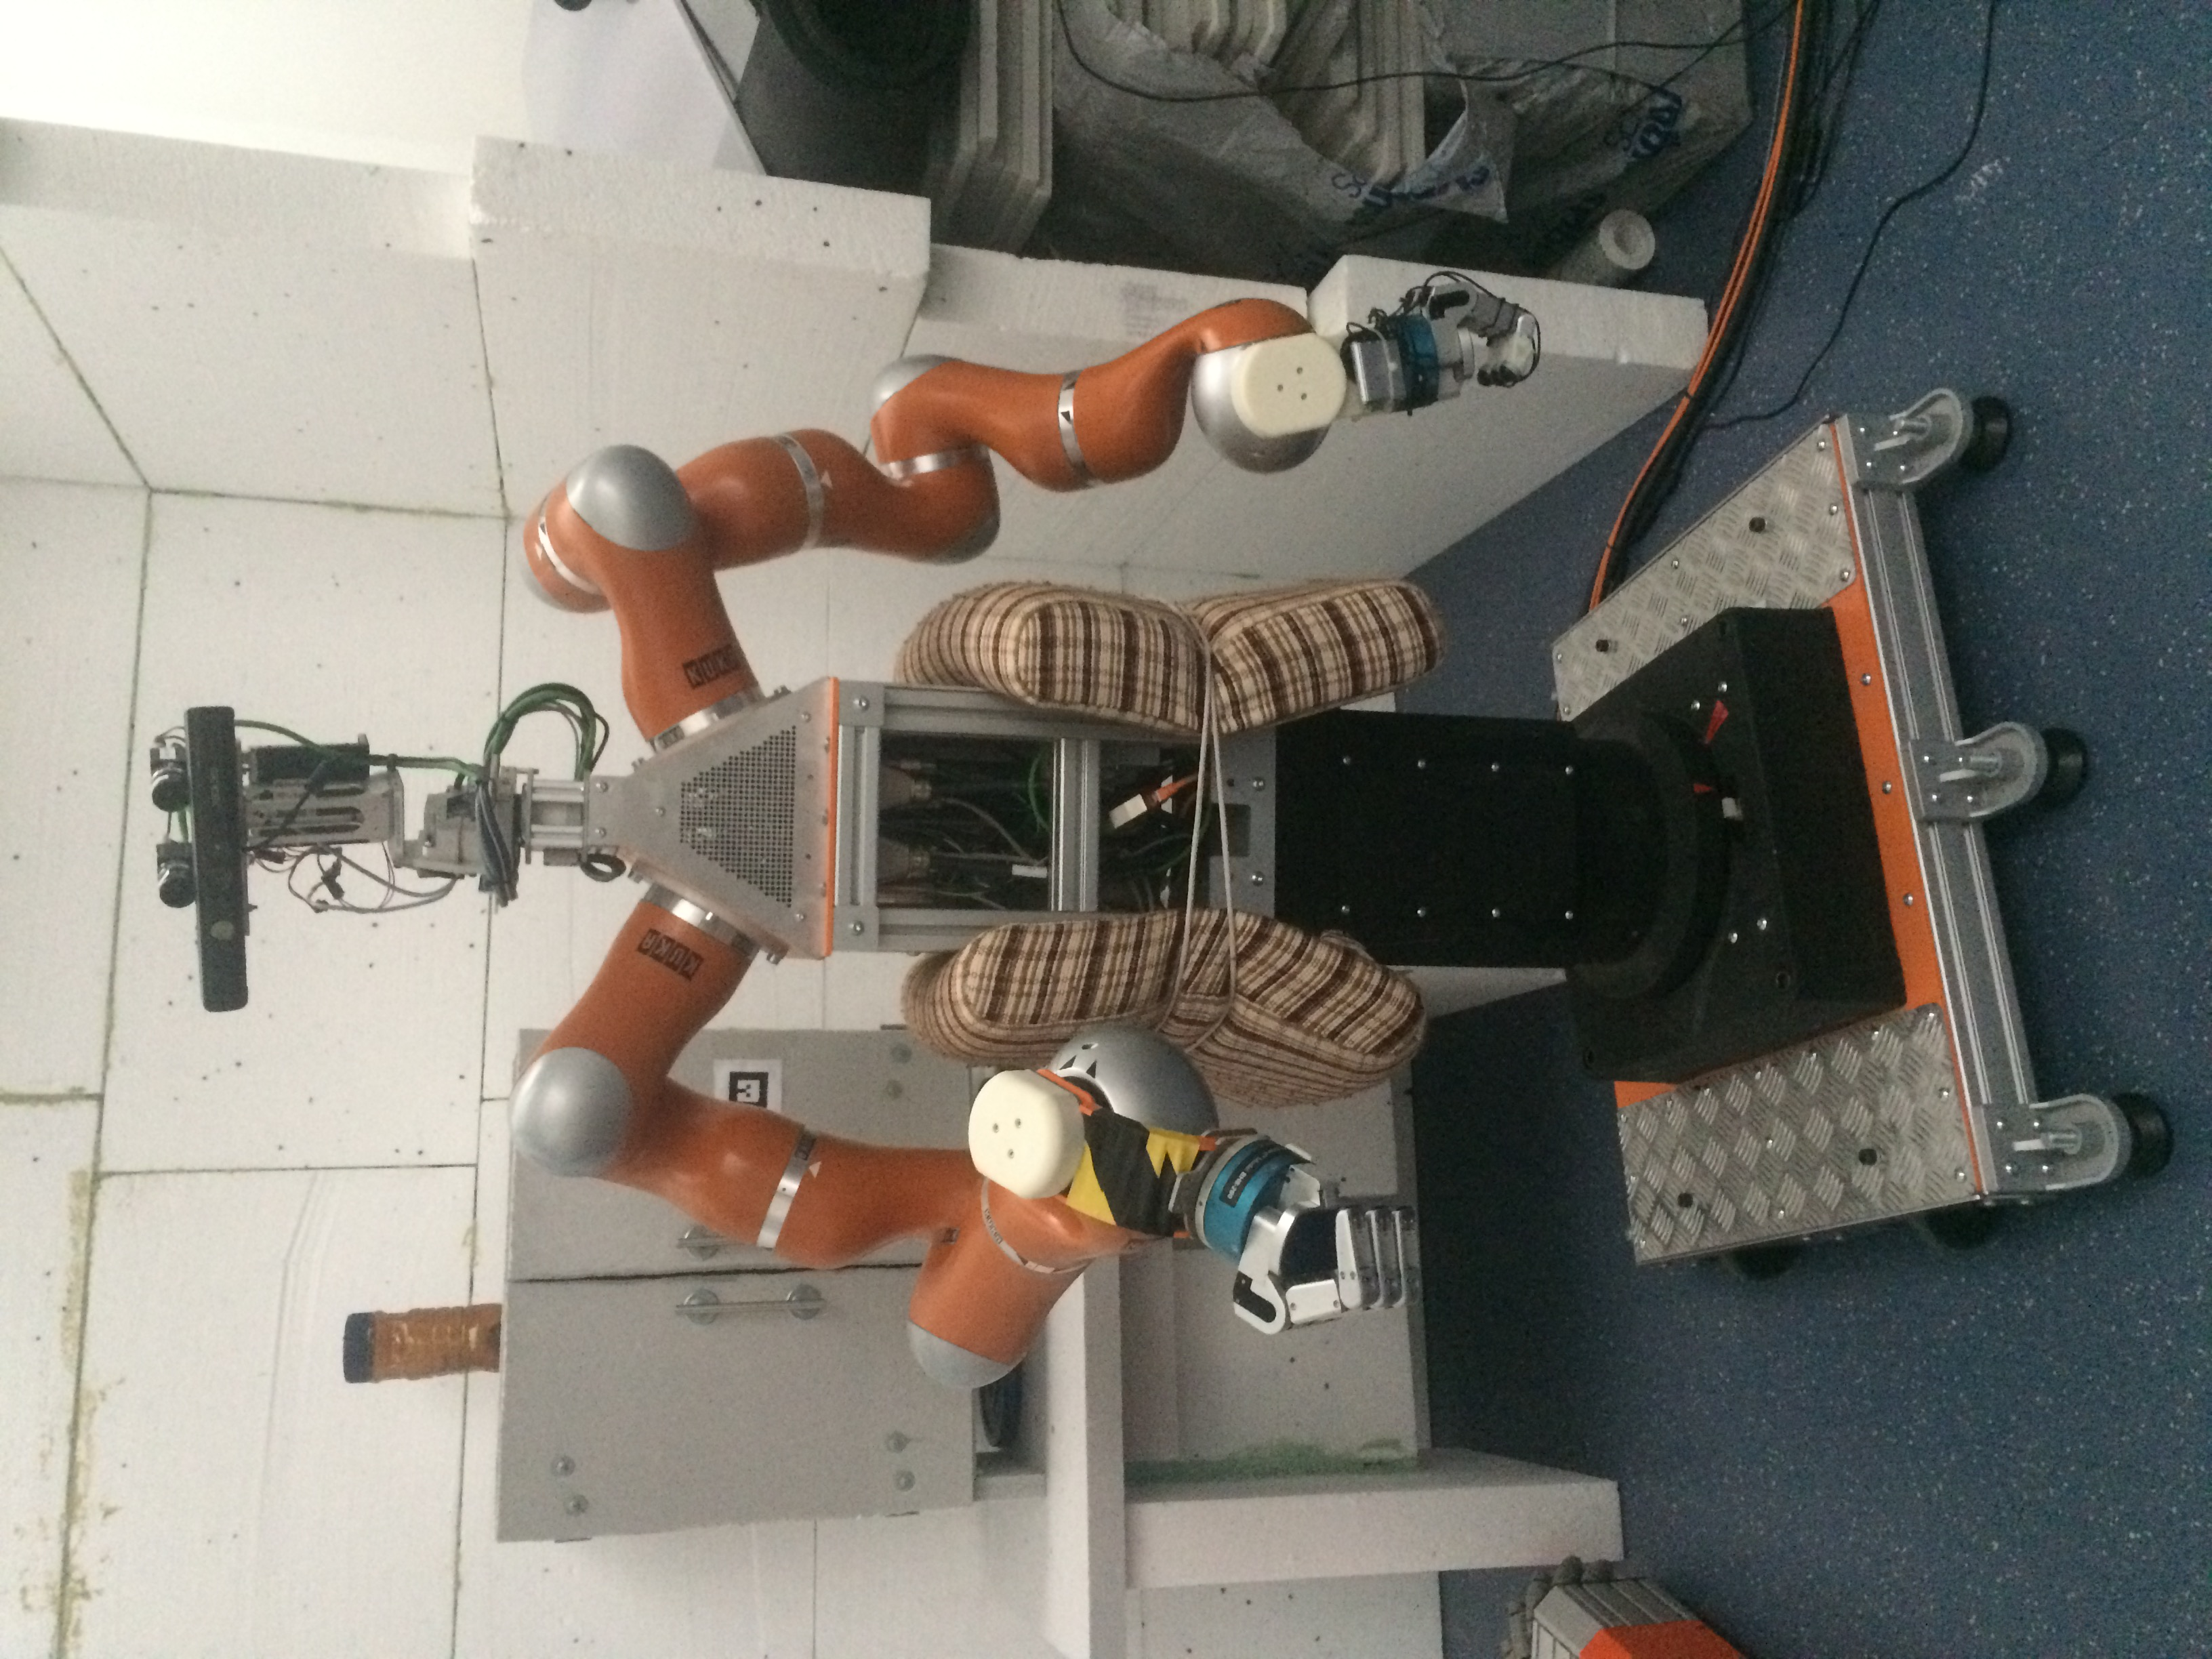
\includegraphics[width=.4\textwidth]{images/velma1.jpg}
		}
		\hfill
		\subfigure[Układy współrzędnych stawów. Najniższy układ współrzędnych obrazuje przyjęty układ odniesienia dla całego systemu. Osie $X$, $Y$ i~$Z$ oznaczone są odpowienio kolorem czerwonym zielonym i~niebieskim\cite{bib:velma2}.]{
			\label{fig:velma2}
			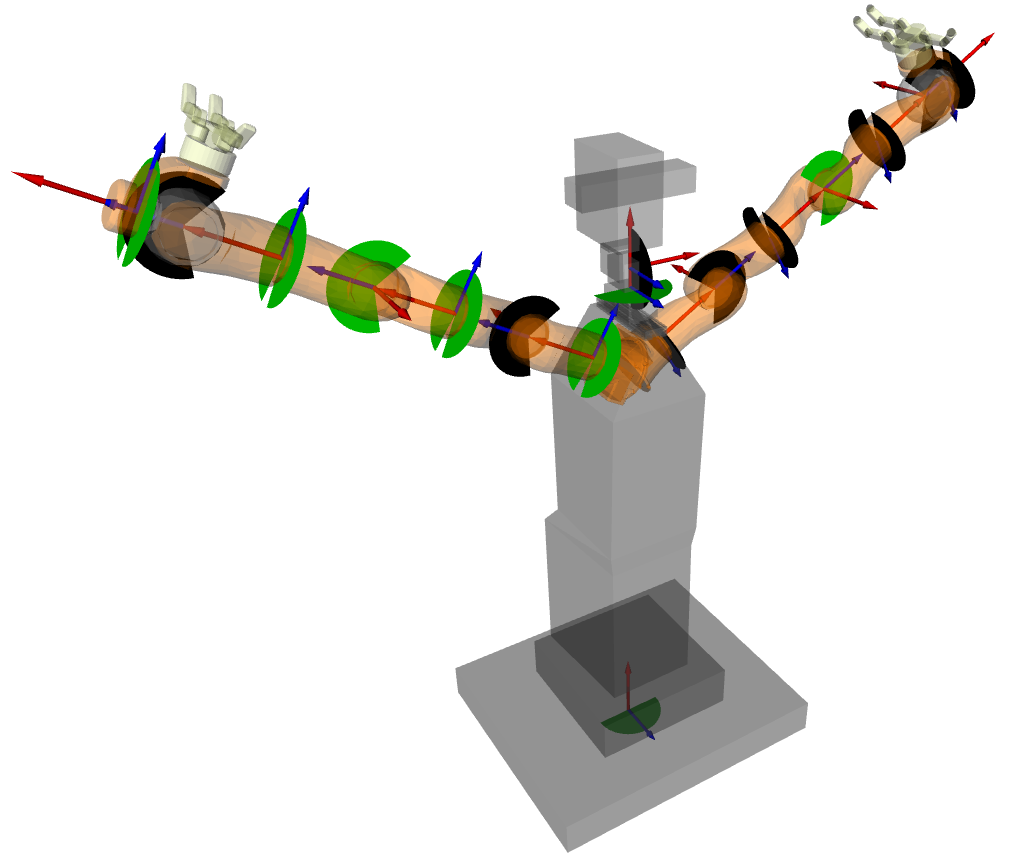
\includegraphics[width=.55\textwidth]{images/velmajoints.png}
		}
		
		\caption{Robot usługowy Velma}
		\label{fig:velma}
		
	\end{figure}
	
\section{Agenty}
System sterowania \cite{bib:velma2} zbudowany jest z~dwóch agentów (rys. \ref{fig:agent}). Agent \textit{velma\_core} jest odpowiedzialny za kontrolę zadań związanych z~manipulacją w~przestrzeni operacyjnej i~konfiguracyjnej robota. Drugi z~agentów \textit{velma\_task\_cs\_ros\_interface} jest interfejsem pomiędzy programami użytkownika pisanymi w~ROS oraz agentem \textit{velma\_core}. Zawiera tylko jeden podsystem o~tej samej nazwie. Użytkownikom został udostępniony dodatkowy interfejs \textit{VelmaInterface} napisany w Pythonie. Nie  jest on częścią agenta \textit{velma\_task\_cs\_ros\_interface} i służy jedynie jako pomoc przy komunikacji z agentem z poziomu programów użytkownika.

Podsystem \textit{velma\_core\_cs} agenta \textit{velma\_core} wylicza prawa sterowanie oraz zajmuje się interpolacją trajektorii. Podsystem \textit{velma\_core\_ve\_body} kontroluje bazowe zachowania bezpieczeństwa. Są to ograniczenia prądowe, wykrywanie krańcowych położeń stawów oraz wykrywanie kolizji. Podsystem przekazuje też sterowanie do efektorów. Podsystemy w~najniższej warstwie abstrakcji mogą być stosowane wymiennie. Do pracy w~rzeczywistym świecie uruchamiane są podsystemy \textit{velma\_core\_re\_lwr\_r} i~\textit{velma\_core\_re\_lwr\_l} oraz podsystem \textit{velma\_ec\_driver}. Służą odpowiednio do kontroli prawego i~lewego ramienia LWR-4 oraz pozostałego sprzętu połączonego magistralą EtherCAT. Do pracy w~trybie symulacji podsystemy w~najniższej warstwie abstrakcji są wymieniane na podsystem \textit{velma\_sim\_gazebo}, w~którym uruchamiany jest symulator świata Gazebo. Podsystem symuluje pracę wszystkich trzech podsystemów odpowiedzialnych za komunikację ze sterownikami sprzętu. 

\begin{figure}
	\centering
	\subfigure[Tryb pracy ze sprzętem]{
		\label{fig:agent_hw}
		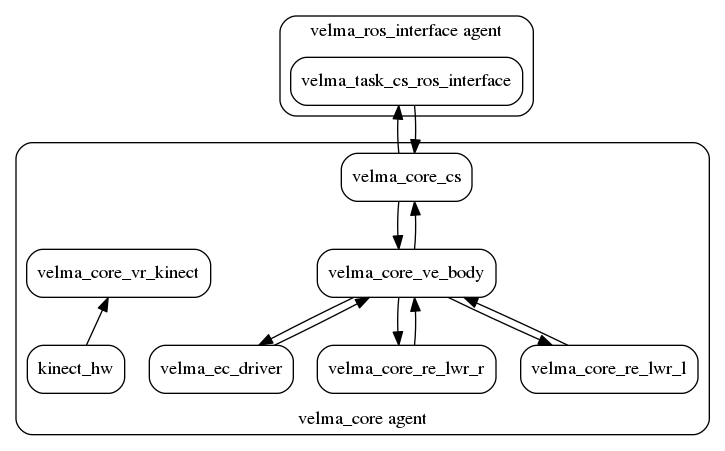
\includegraphics[width=.72\textwidth]{images/system_hw.png}
	}
	\hfill
	\subfigure[Tryb symulacji]{
		\label{fig:agent_sim}
		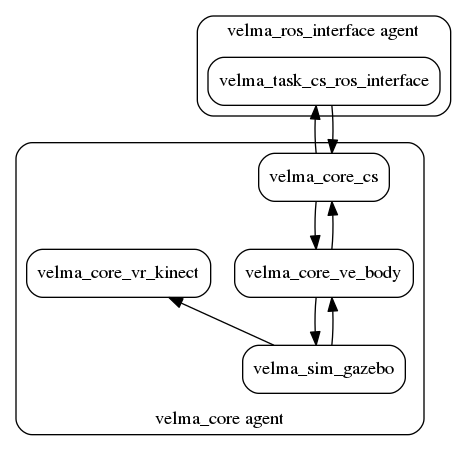
\includegraphics[width=.45\textwidth]{images/system.png}
	}
	
	\caption{Poglądowy i~uproszczony schemat agentów robota Velma zawierający także nieopisywane części systemu odpowiedzialne za nadzór Kinecta\cite{bib:velma2}.}
	\label{fig:agent}
	
\end{figure}


\begin{itemize}
	\item \textbf{Interfejs akcji ROS} - 
	Komponent \textit{CartImpActionRight} znajduje się w~podsystemie \textit{velma\_task\_cs\_ros\_interface} i~odbiera rozkazy wysłane przez użytkownika przez mechanizm akcji ROS oraz przesyła je do innych podsystemów. Zwraca też status wykonania operacji. Komponent służy do obsługi prawego ramienia i~istnieje analogiczny komponent \textit{CartImpActionLeft} służący do obsługi lewego ramienia.
	\item \textbf{Publikacja wektorów pozycji} - 
	Komponent \textit{TfPublisher} wysyła do użytkownika za pomocą ROSa położenie i~obrót istotnych dla działania systemu miejsc robota takich jak chwytaki czy środek ciężkości korpusu. 
	\item \textbf{Pozycje stawów} - 
	Odczyt pozycji stawów jest zależny od trybu pracy oprogramowania. Jeśli używamy trybu obsługi rzeczywistego sprzętu to za odczyt pozycji są odpowiedzialne podsystemy \textit{velma\_core\_re\_lwr\_r} i~\textit{velma\_core\_re\_lwr\_l} oraz podsystem \textit{velma\_ec\_driver}, które posiadają pojedyncze komponenty służące do komunikacji z~fizycznymi sterownikami magistral. W~trybie symulatora emulacją tych trzech podsystemów zajmuje się podsystem \textit{velma\_sim\_gazebo}, który jako symulator nie jest podzielony na konkretne podsystemy.
	\item \textbf{Zadawanie momentów} - 
	Zadawanie momentów obrotowych w~stawach następuje w~analogiczny do odczytywania pozycji sposób.
	\item \textbf{Kinematyka prosta} - 
	Komponent \textit{FK} pobiera dane o~pozycjach stawów i~wylicza pozycję chwytaka oraz innych części robota.
	\item \textbf{Interpolator trajektorii} - 
	Komponent \textit{INT\_tool\_r} z~podsystemu \textit{velma\_core\_cs} odpowiada za interpolacje trajektorii zadanej prawemu ramieniu. Interpolator służy temu by jedno polecenie przesunięcia ramienia zamienić na wiele mniejszych i~rozłożonych w~czasie. W~konsekwencji algorytm sterowania nie jest narażony na duże uchyby a~ruch ramienia jest wykonywany płynnie. Do działania komponent potrzebuje aktualnych i~zadanych pozycji. Komponent służy do obsługi prawego ramienia. Analogicznie do obsługi lewego ramienia służy komponent \textit{INT\_tool\_l}.
	
	\item \textbf{Prawo sterowania impedancyjnego} - 
	Komponent \textit{cart\_imp} z~podsystemu \textit{velma\_core\_cs} służy do wyliczania momentów zadawanych na stawy zgodnie z~algorytmem prawa sterowania impedancyjnego w~przestrzeni kartezjańskiej. Pobiera zadaną pozycję z~interpolatora trajektorii.
\end{itemize}

	\section{Pakiety oprogramowania}
	\subsection{ROS}
	Struktura ramowa ROS (Robot Operating System)\cite{bib:ROS} zapewnia biblioteki usprawniające pisanie programów dla robotyki w~C++ i~Pythonie. Pozwala na komunikację pomiędzy programami na zasadzie tematów oraz na zasadzie usług. Posiada gotowe funkcje wspomagające obliczenie kinematyki oraz wizualizujące ważne parametry pracy robota. Kolejnym narzędziem jest \textit{rviz}, który wizualizuje stawy robota wraz z układami współrzędnych. Pakiet daje możliwość akwizycji danych. Podstawowymi narzędziami w~pakiecie są:
	\begin{itemize}
		\item \textbf{Węzły} - Programy pisane w~C++ lub Pythonie spełniające zdefiniowaną w~systemie funkcję.
		\item \textbf{Serwisy} - Usługi udostępniane przez węzły pozwalające na komunikację w~architekturze zapytanie-odpowiedź. Każdy program może udostępniać wiele serwisów. Służą do wywoływania zdalnych procedur.
		\item \textbf{Akcje} - Usługi podobne do serwisów lecz nieblokujące wykonywania węzła będącego serwerem.
		\item \textbf{Tematy} - Usługi udostępniane przez węzły pozwalające na asynchroniczną komunikację. Każdy program może udostępniać i~pobierać wiele tematów. Służą do aktualizowania bieżącego stanu całego systemu.
		\item \textbf{Zarządca} - Odpowiada za komunikację i~nadzoruje pracę innych narzędzi pakietu.
	\end{itemize}
	\subsection{Orocos}
	Orocos \cite{bib:Orocos} jest wolnym oprogramowaniem napisanym w~C++ służącym do tworzenia aplikacji zgodnych z~wymaganiami czasu rzeczywistego. Pozwala na implementację  oprogramowania w~podejściu komponentowym. Zestaw bibliotek pakietu Orocos składa się między innymi z:
	\begin{itemize}
		\item \textbf{RTT (ang. Real-Time Toolkit)} - Biblioteki służące do  tworzenia komponentów w~aplikacjach czasu rzeczywistego.
		\item \textbf{OCL (ang. Orocos Component Library)} - Biblioteki pomocne w~trakcie uruchamiania komponentów.
		\item \textbf{OroGen} oraz \textbf{TypeGen} - Narzędzia do automatycznego generowania komponentów i~typów danych.
		\item \textbf{Deployer} - Uruchamia komponenty zgodnie z~opisem zawartym w~pliku XML oraz pozwala na nadzór tych komponentów trakcie pracy.
	\end{itemize}

	\subsection{FABRIC}
	Framework for Agent–Based Robot Control Systems - FABRIC\cite{bib:fabric} wykorzystuje Orocosa oraz strukturę ramową ROS zapewniając interfejs programistyczny pozwalający na tworzenie komponentów zgodnych z~założeniami teorii agentowej. Ma zaimplementowane algorytmy komunikacji pomiędzy poszczególnymi podsystemami poprzez zdefiniowane wiadomości. Posiada narzędzie wizualizujące stan predykatów, zachowań i~podsystemów \textit{rqt\_agent}\cite{bib:rqtAgent}. Pokazuje też przepływ danych między komponentami.

	
	\section{Symulator robota}
	Symulator robota Velma jest wytworzony w~oprogramowaniu Gazebo \cite{bib:Gazebo} które symuluje obiekty i~zachowania między nimi zgodnie z~prawami fizyki. Użytkownik ma możliwość zdefiniowania całego środowiska wraz z~robotem (rys. \ref{fig:gazebo}). Posiada gotowe modele wielu receptorów i~efektorów oraz pozwala na tworzenia własnych. Daje możliwość emulowania sterowników sprzętu. Interfejs użytkownika udostępnia opcję wywarcia siły bądź momentu na dowolny przedmiot będący w~symulacji. Emuluje czas, jeśli symulacja nie jest przeprowadzana w~czasie rzeczywistym.
	
	\begin{figure}
		\centering
		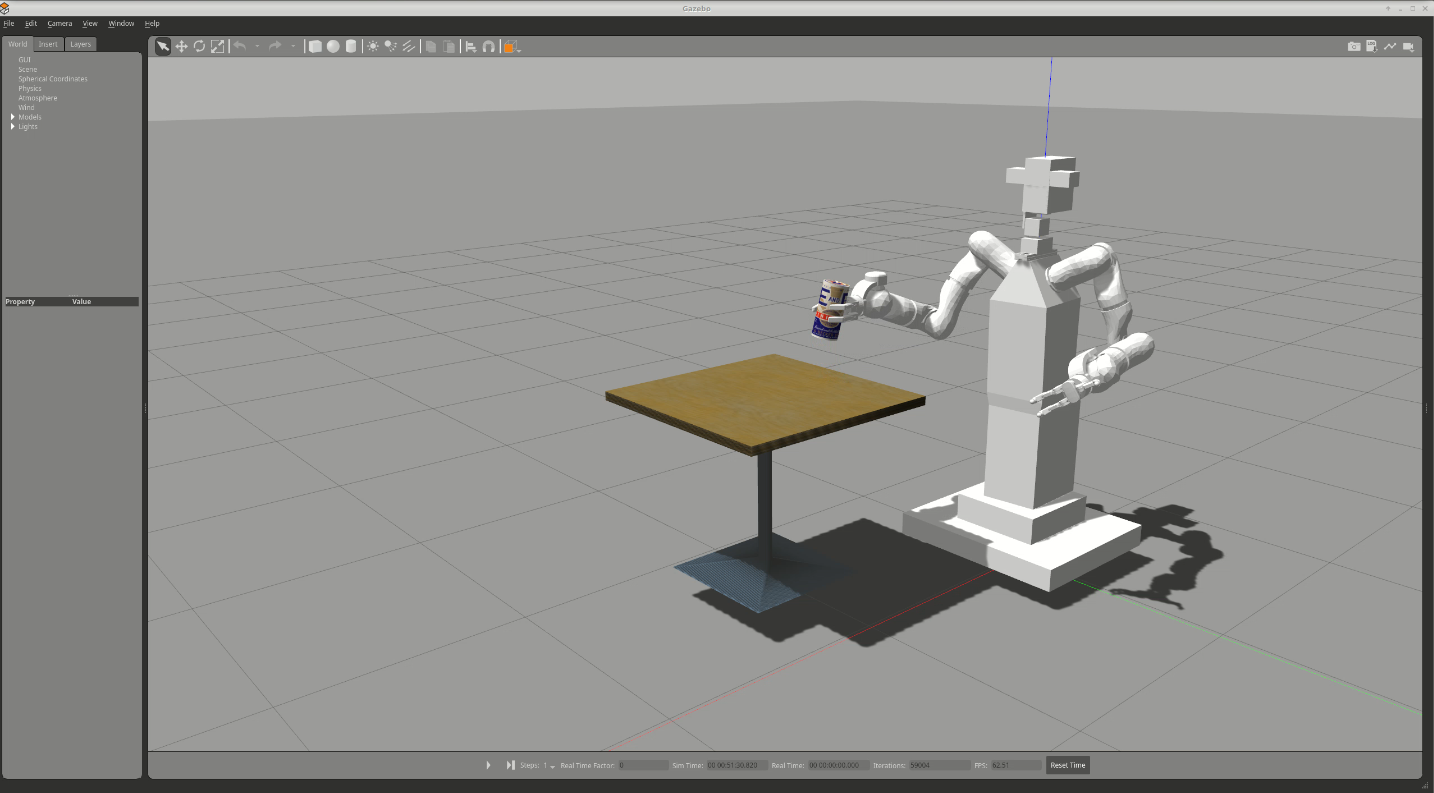
\includegraphics[width=.6\textwidth]{images/gazebo.png}
		\caption{Robot Velma w~trakcie manipulacji. Symulacja w~środowisku Gazebo.}
		\label{fig:gazebo}
	\end{figure}

	Oryginalny kod Gazebo został przystosowany do pakietu oprogramowania DART (ang. Dynamic Animation and Robotics Toolkit) \cite{bib:dart} symulującego fizykę zdefiniowanego świata. Pakiet DART został wybrany przez Zespół Programowania Robotów i~Systemów Rozpoznających, ponieważ po jego zastosowaniu został wyeliminowany problem narastających oscylacji członów robota w~trakcie symulacji. W~przeciwieństwie do wielu symulatorów fizyki DART daje dostęp do wielu przydatnych informacji takich jak jakobian bądź macierz inercji przedmiotów. Zastosowano~w nim algorytm LCP (ang. Linear Complementarity Problem), \cite{bib:lpcBase} który sprowadza model fizyczny świata do zestawu równań kwadratowych. DART symuluje działanie wielu sił w~tym siły Coriolisa i~tarcia dynamicznego. Dzięki temu możliwe jest zaawansowane wykrywanie kolizji. 
	
	